%%%%%%%%%%%%%%%%%%%%%%%%%%%%%%%%%%%%%%%%%%%%%%%%%%%%%%%%%%%%%%%%%%%%%%%%%%%%%%%%
%2345678901234567890123456789012345678901234567890123456789012345678901234567890
%        1         2         3         4         5         6         7         8

\documentclass[letterpaper, 10 pt, conference]{ieeeconf}  % Comment this line out if you need a4paper

%\documentclass[a4paper, 10pt, conference]{ieeeconf}      % Use this line for a4 paper

\IEEEoverridecommandlockouts                              % This command is only needed if you want to use the \thanks command

\overrideIEEEmargins                                      % Needed to meet printer requirements.

% See the \addtolength command later in the file to balance the column lengths
% on the last page of the document

% The following packages can be found on http:\\www.ctan.org
\usepackage{graphicx} % for pdf, bitmapped graphics files
\usepackage{subcaption}
%\usepackage{epsfig} % for postscript graphics files
%\usepackage{mathptmx} % assumes new font selection scheme installed
%\usepackage{times} % assumes new font selection scheme installed
%\usepackage{amsmath} % assumes amsmath package installed
%\usepackage{amssymb}  % assumes amsmath package installed

\title{\LARGE \bf
Movie Rating Prediction Using Nonnegative Matrix Factorization on Movie Tags
}


\author{Claire Chang, Thaxter Shaw, and TJ Tsai$^{1}$% <-this % stops a space
\\ \vspace*{10pt} \normalsize  May 14, 2021

\thanks{$^{1}$T. Tsai is with the Department of Engineering at Harvey Mudd College,
301 Platt Blvd., Claremont, CA 91711. E-mail: {\tt\small ttsai@hmc.edu}}%
}



\begin{document}



\maketitle
\thispagestyle{empty}
\pagestyle{empty}


%%%%%%%%%%%%%%%%%%%%%%%%%%%%%%%%%%%%%%%%%%%%%%%%%%%%%%%%%%%%%%%%%%%%%%%%%%%%%%%%
\begin{abstract}

The goal of recommendation systems is to suggest suitable content such as movies or groceries. This article aims to predict what someone will rate a movie, which could in turn be applied to a movie recommendation system.
We investigate this problem using 1,024 movies and 204,924 ratings from a MovieLens dataset.
We address this problem using nonnegative matrix factorization (NMF). This original method produced a root mean square error (RMSE) of 0.9748. We then propose a mechanism to improve these predictions by rounding our preliminary rating prediction based on the mean movie rating.
Our improved method achieves an RMSE of 0.9597. This RMSE is significantly better than the RMSE of 0.9644 for a naive system that simply predicts the mean movie rating.

\end{abstract}


%%%%%%%%%%%%%%%%%%%%%%%%%%%%%%%%%%%%%%%%%%%%%%%%%%%%%%%%%%%%%%%%%%%%%%%%%%%%%%%%
\medbreak
\section{INTRODUCTION}

Suppose you are on Netflix and have just finished the latest season of your favorite show. Now, you need to find something new! But luckily, you discover that there is a show that looks interesting being recommended to you. After watching a few episodes, you fall in love. How did this process work? This is the problem behind recommendation systems. 

In this paper, we will try to predict what someone will rate a movie on a five-star scale. This prediction can be used in recommendation systems for not only movies or shows, but also grocery shopping, music, and more \cite{recsys}. One type of approach that has been taken is to use a ``neighborhood approach" that compares different movies, and recommends a highly rated movie that is similar to other movies a user has liked. 
Another type of approach is to use collaborative filtering methods such as nonnegative matrix factorization (NMF) and singular value decomposition (SVD) \cite{cf}. 
It is also possible to use a hybrid approach of the neighborhood and collaborative filtering approaches \cite{hybrid}. Our paper will focus on collaborative filtering methods, and more specifically, on NMF. However, it is worth noting that hybrid approaches tend to perform better \cite{netflix}.

Previous works \cite{nmfratings} have used NMF to describe the reviewer rating matrix in a recommendation system, and found that NMF-based algorithms obtain the best performance in certain situations when compared with other collaborative filtering methods. More directly comparing NMF with other collaborative filtering methods, it has been shown \cite{nmfratings} that NMF is more sensitive to initial conditions. Other works \cite{cfcompare} have also looked into comparing NMF with other collaborative filtering methods, and found that SVD results in better accuracy (unless there are a relatively low number of users and items), but also requires more computation time. For example, one successful team using modified SVD algorithms on the Netflix dataset (containing 480,189 reviewers and 17,770 movies) won the 2007 Netflix Progress Prize \cite{netflix}. Besides accuracy and runtime, there are also trade-offs with using a larger dataset and using SVD. Although they are more accurate, these algorithms tend to also have a higher variance in accuracy and be less computationally efficient \cite{cfcompare}.

In this paper, we use data from a MovieLens dataset. The subset of the dataset we use contains ratings 1,024 movies made by various users, filtered such that each user has rated at least 20 movies.
The dataset also relates each movie to a series of short tags, such as ``sci-fi," ``cliché," or ``overrated." This data was collected through users applying labels to movies, and machine learning \cite{lenskitdata}. Another challenge presents itself in the tags. We can sort the tags into categories such as movie type (for example, romance or comedy) and a user or subjective view (for example, funny or boring) \cite{tags}. While the subjective tags with a positive sentiment more clearly correspond with a generally highly rated movie, the other tags are a bit more complex. In particular, subjective tags with a negative sentiment may be detrimental to our prediction system, which we will discuss in more detail later.


Our system uses NMF on this tag data to create clusters of tags, which we will equate to ``genres." We use NMF due to time and space constraints, and because using a smaller set of data means that NMF should perform relatively better than other collaborative filtering methods \cite{cfcompare}.  After performing NMF, we leverage the genres to predict ratings. Finally, we take mean movie ratings into account in order to adjust these predicted ratings.

There are two key differences between our approach and other works. First, we use NMF on tag data. By contrast, previous works have used NMF on ratings directly \cite{nmfratings}. This difference allows us to consider smaller details about movies and thus make more connections between them. This change relies on the assumption that the tags are a good measure of the movie's content and adequately model how a reviewer will feel about the movie. Second, we make informed adjustments to our predictions based on the mean movie ratings. This adjustment allows us to consider both user preferences (from NMF) and overall movie quality (from the movie mean rating). With our adjustment, we obtain a root mean square error of 0.9597.

\medbreak
\section{SYSTEM DESCRIPTION}

Our system's design is illustrated in Figure 1. There are three key components that are needed to construct this system: performing NMF, creating an ``expectation" for user preferences, and generating a rating prediction. These steps are described in detail in the following three subsections.

\begin{figure}[h]
   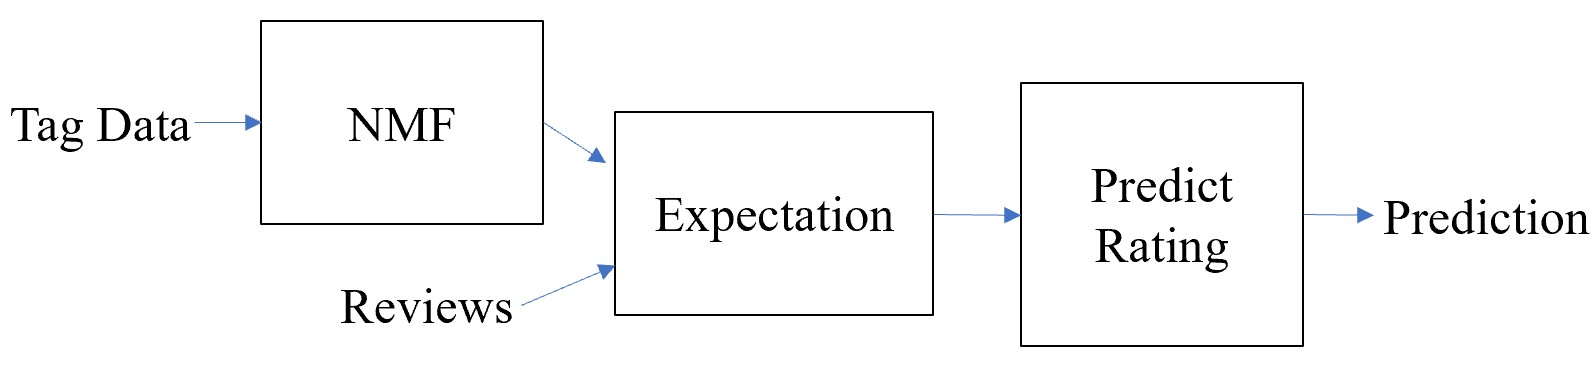
\includegraphics[scale=0.5]{./figs/blockdiagram.jpg}
   \caption{Block diagram of proposed system.}
\end{figure}

\smallbreak
\subsection{Nonnegative Matrix Factorization}

We begin with the tag data, stored as a matrix of $t$ rows and $m$ columns. Here, $t$ is the number of tags and $m$ is the number of movies in the dataset.
We perform NMF on the tag data matrix with $R=50$ templates, which gives us a template matrix $W_{t \times R}$ and an activation matrix $H_{R \times m}$. 

Each template is comprised of clusters of tags and represents a genre. For example, the romantic comedy genre might contain the tags ``cliché," ``romance," ``Ryan Gosling," and ``comedy." Hence $H$ represents how each movie is broken down into its component genres.

It is important to mention that we use a random initialization for $W$ and $H$. Ideally, we would want to discount negative subjective tags by setting corresponding entries in the $W$ initialization to 0 (so that if someone happened to love some movies that were tagged ``not funny," they would not express a preference towards other ``not funny" movies). However, this task is challenging because it requires either manually reviewing each of the 1,128 tags or performing some sort of sentiment analysis. For simplicity, we make the (perhaps dangerous) assumption that there are not too many negative tags, or that the negative tags are mainly associated with movies with low ratings.

While experimenting with our system design, one of the parameters we tried to vary was the number of templates used in NMF ($R$). We noticed that from 10 to 50 templates, there was noteworthy increase in performance and a comparable runtime. By contrast, when testing between 50 and 1000 templates, performance remained about the same despite significant increases in runtime. Therefore, we decided to use 50 templates.

\smallbreak
\subsection{Expectation}

Next, we assemble a new matrix of reviews. This matrix stores all ratings made by each user. It has $m$ rows and $p$ columns, where $p$ is the number of reviewers.

Then, we create another matrix, $M_{R \times p}$, which represents each reviewer's affinity to each genre. Each entry in $M$ is a rating out of five stars indicating what a reviewer is expected to rate a typical movie from a given genre.
We get an entry in $M$ by taking the ``expectation" of all the reviewer's ratings. To calculate this expectation, we use values in $H$ to weigh ratings in the reviews matrix. In this way, ratings of movies more relevant to the genre of interest are given more weight.

\subsection{Predict Rating}
Finally, we generate a predicted rating for a movie and reviewer from a query. For example, suppose we want to predict what Reviewer A will rate the movie \textit{La La Land}. To do this, we will use a ``genre fingerprint" for our movie.

Recall that $H$ is an $R \times m$ matrix storing the relevance of each genre to each movie. We can L1 normalize the columns of $H$ to create a matrix storing the genre fingerprints of each movie.
These fingerprints indicate the breakdown of the movie into its component genres, such that each genre represents a proportion of the entire movie. See Figure 3 for examples of genre fingerprints.

For our example, let's assume that \textit{La La Land}'s fingerprint consists of 75\% romantic comedy and 25\% drama. Then, based on Reviewer A's preferences for these genres (from matrix $M$), we can generate a preliminary prediction for their rating. 75\% of this prediction will be based on Reviewer A's predilection towards the romantic comedy genre, and 25\% of it will come from the drama genre.
Note that this example is extremely simplified. In our actual system, the movie fingerprints are much more complex (as we can see in Figure 3). In the next section, we will see that these preliminary predictions are somewhat flawed. Therefore, we will introduce an additional step to adjust the prediction.

For our adjustment, we wish to take movie quality into account. If the movie's mean rating is higher than our preliminary prediction, we round up to the nearest half-star. Otherwise, we round down. However, there is the caveat that this rounding is a somewhat basic way of balancing user preferences and overall movie quality. Thus, for a more complex system, we may wish to add a hyperparameter that modifies the weights of the two factors.

\medbreak
\section{RESULTS}

For our experiments, we use the ratings from the first 1,024 movies from the MovieLens dataset and the relevance of those movies to each of the 1,128 tags. The 204,924 available ratings were divided into an 80\% training and 20\% testing split, and the system was applied to the training cases to make predictions for test cases \cite{lenskitmodule}. We can see the rating distribution of the training data in Figure \ref{ratingdist}. We expect the distribution to reflect those of the testing and overall dataset. 

As is common in collaborative filtering problems, we use the Root Mean Square Error (RMSE) as an evaluation metric \cite{lenskitmodule}. RMSE is calculated as follows: 
$$\sqrt{\frac{\sum_{i=1}^N (x_i - \hat{x}_i)^2}{N}},$$
where $N=40,984$ is the number of ratings in the testing set, $x_i$ is the actual rating, and $\hat{x}_i$ is our predicted rating. Note that the training and test splits are randomized, which could cause some minor variation in results. We will share results for one particular instance, but the predictions should be relatively similar across different splits.

\begin{figure}[h]
    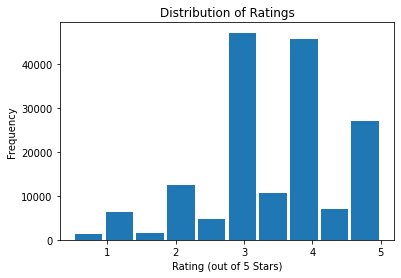
\includegraphics[scale=0.6]{figs/ratingdist.png}
    \caption{Distribution of ratings for the training dataset. We can see that most of the ratings are 3 and 4 stars.}
    \label{ratingdist}
\end{figure}

As a baseline, the RMSE when predicting the mean movie rating was 0.9644. Before implementing the rounding mechanism, the RMSE with our algorithm was about 0.9748. We noticed that even the RMSE with the mean was better, but thought that our system was considering different factors--namely, the tags. Additionally, we suspected there could be some error if, for example, we predicted 3.6 stars as a rating but the true rating was 3.5 stars. Thus, we decided to round our prediction using the mean as an indicator. After adding the rounding, the RMSE decreased to approximately 0.9597. 

As mentioned earlier, we may wish to add a hyperparameter that modifies the weights of the mean movie rating and user preferences (NMF results) in order to create a more nuanced system. From Figure \ref{ratingdist}, it is also interesting to note that half-star ratings are less popular. One reason may be that people prefer giving whole numbers, and ratings of 1, 2, 3, 4, and 5 stars adequately describe their opinions about movie quality. In the future, we could explore the effect of discouraging half-star ratings.

There are a few observations we can make about these results. First, we can study the genre fingerprint for the most and least accurate predictions. The difference between our predicted rating and the true rating was 0 stars for the accurate rating, and 4 stars for the inaccurate rating. Referencing Figure 3, we notice that in the case of the accurate rating, the most prominent genre represents about 30\% of the movie, and all other genres comprise 15\% or less. On the other hand, for the inaccurate rating, the most prominent genre only represents about 14\% of the movie, and there are five other peaks between 8\% and 10\% alone.

\begin{figure}[h]
   \begin{subfigure}[b]{\columnwidth}
      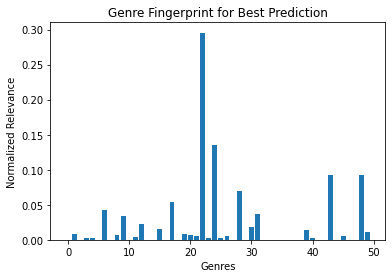
\includegraphics[width=\linewidth]{./figs/bestfingerprint.png}
      \caption{Fingerprint of movie from good prediction.}
   \end{subfigure}
   \hfill
   \begin{subfigure}[b]{\columnwidth}
      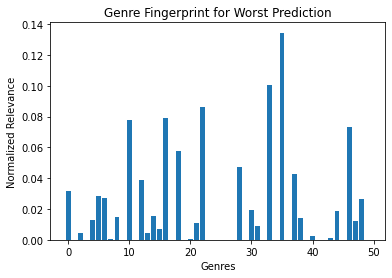
\includegraphics[width=\linewidth]{./figs/worstfingerprint.png}
      \caption{Fingerprint of movie from bad prediction.}
   \end{subfigure}
   \caption{Fingerprints of two movies. A fingerprint is the breakdown of the movie into genres. We can see that the fingerprint of the movie from the bad prediction has a wider distribution.}
\end{figure}

From Figure 3, we hypothesize that our system performs better when a movie's categorization is more straightforward, and it falls primarily into a single genre. If the movie breaks down into several genres, it is more difficult to predict a rating. What if there are two high peaks, and the reviewer loves one of the genres and hates the other one? In this case, our system would predict a medium review, but it is more likely that the reviewer would either give a high or a low rating. We attempted to address this concern by only using the most significant genre, but this approach had a very high RMSE of approximately 1.003. This failure is potentially because the true rating could just as easily reflect the secondary or tertiary genre of a movie, rather than the primary one.

We also considered filtering out less relevant genres, but the variation in normalized relevance made this problematic. Instead, we tried filtering tags. If the total tag relevance across all movies was under a certain amount, we ignored that tag by setting its initialization in the $W$ matrix to 0 for NMF. Running our algorithm with this modification (but without the rounding adjustment) produced an RMSE of about 0.9739. This result is comparable the RMSE of 0.9748 when running without this modification. One reason this filtration was not effective might be because the relevance of the tags does not matter as much as their meaning. As mentioned previously, another step could be to filter negative tags.

Besides the genre fingerprint, we can look at the distribution of ratings across all reviewers for these accurate and inaccurate predictions. Referencing Figure 4, we can see that for the ``good prediction," there is a clear peak at 3 stars. As you might expect, both our predicted rating and the true ratings were 3 stars. If we look at the ``bad prediction," there are peaks at 4 and 5 stars. We predict a rating of 4.5 stars, which seems to be reasonable. However, the reviewer in question gave a 0.5 star rating.

\begin{figure}[h]
   \begin{subfigure}[b]{\columnwidth}
      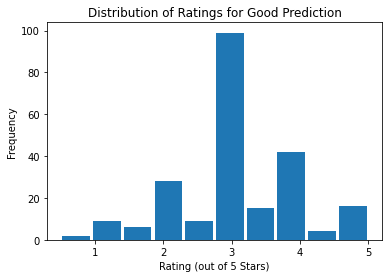
\includegraphics[width=\linewidth]{./figs/gooddist.png}
      \caption{Distribution of ratings for a well-predicted movie. The predicted and true ratings were both 3.0 stars.}
   \end{subfigure}
   \hfill
   \begin{subfigure}[b]{\columnwidth}
      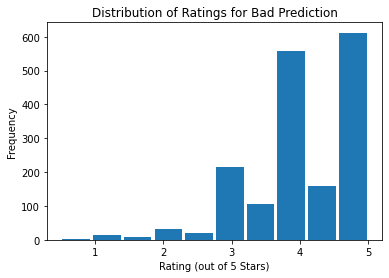
\includegraphics[width=\linewidth]{./figs/baddist.png}
      \caption{Distribution of ratings for a badly-predicted movie. The predicted and true ratings were 4.5 and 0.5 stars respectively, while the most popular ratings seem to have been 4.0 and 5.0 stars.}
   \end{subfigure}
   \caption{Rating distributions for two movies.}
\end{figure}

From Figure 4, we hypothesize that there may be anomalies or outliers in our system caused by untracked factors or other unforeseeable circumstances. Because the RMSE gives more weight to large prediction errors, we can see the results of these anomalies in our error. 

Ultimately, these observations demonstrate that tag data alone may not be sufficient to accurately predict what someone might rate a movie. Our system's dependency on tag data is a major drawback when compared to other systems that consider several factors and hence have lower RMSEs. For example, a study with a hybrid approach investigating temporal effects \cite{netflix} obtained an RMSE of 0.8784. That is, over time, users may change their baseline rating (for example, have higher expectations of graphics) and begin to prefer different genres and actors.
Movies themselves also become more or less popular over time. We do know, however, that an RMSE of between 0.85 and 1.3 or more is to be expected when predicting ratings \cite{netflix}.

\medbreak
\section{CONCLUSION}

We have proposed a method to predict what a reviewer would rate an arbitrary movie out of five stars. To do this, we use the reviewer's history and the movie's relevance to a series of short labels, or tags.
Our approach modifies results from nonnegative matrix factorization (NMF) on the tag data by rounding based on the mean movie rating. We evaluate our system on a dataset of 1,024 movies, and 204,924 ratings.
Our system achieves a root mean square error of 0.9597.
Our underlying assumption is that the tags are a good measure of the movie's content and adequately model how a reviewer will feel about the movie.

One potential area of future work is to handle situations that violate this assumption. For example, we may not want to affiliate users with tags that have negative sentiments. Another area of future work is to add and fine-tune a hyperparameter to find the optimal balance between weights for user preferences (expressed through NMF results) and overall movie quality (from mean movie ratings).


\bibliographystyle{IEEEtran}
\bibliography{paperbib}




\end{document}
